\chapter{Results}

\section{Synthetic Data}

\subsection{Test for Disequilibrium}

\begin{figure}[htbp]
\centering
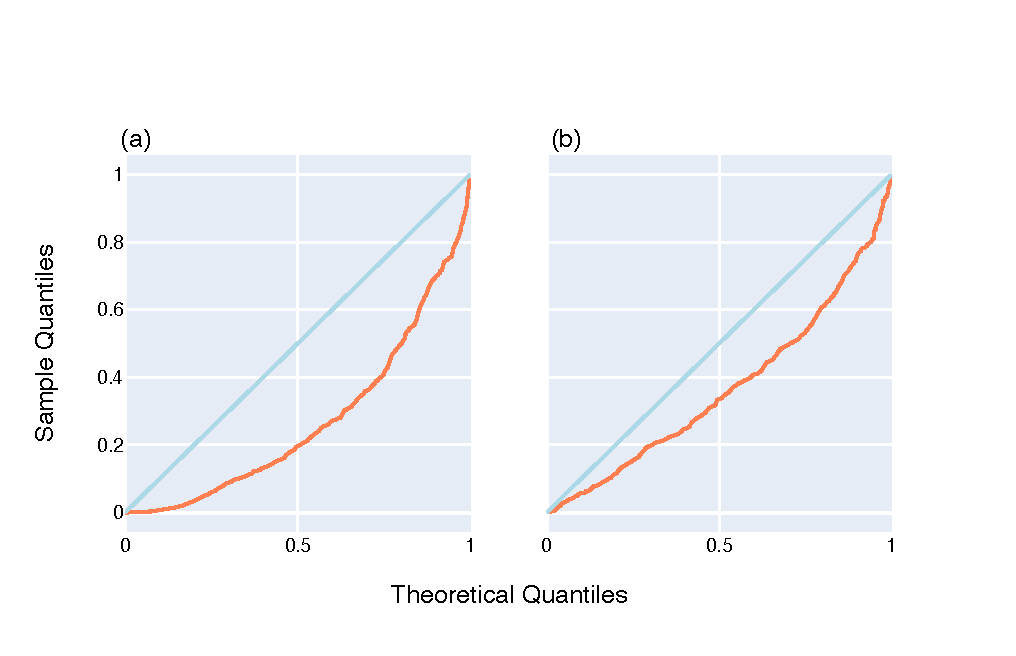
\includegraphics[width=\textwidth]{figures/plots/synthetic/lrt/197113_332182_17210-long_seq.pdf}
\caption[Increasing the length of the alignments gives a distribution of $\hat p-$ values closer, but not consistent with theoretical expectations]{\textbf{Increasing the length of the alignments gives a distribution of $\hat p-$ values closer, but not consistent with theoretical expectations.} The Quantile-Quantile (Q-Q) plots compare the $\hat p$-value distribution of the test for existence in stationary simulated data to the uniform distribution (pink line). Theoretical expectation is illustrated by the diagonal (blue line). Q-Q plot for \textbf{(a)} synthetic alignments of length $300$bp, \textbf{(b)}, synthetic alignments of length $30,000$bp. Each data set contains 1,000 synthetic stationary alignments. Both data sets shown are generated from the same high JSD, high entropy seed. The other seeds exhibited the same pattern, the result is shown in the appendix Figure \ref{fig:synthetic/lrt/all-seeds}.}
\label{fig:synthetic/lrt/197113-long_seq}
\end{figure}

\begin{figure}[!ht]
\centering
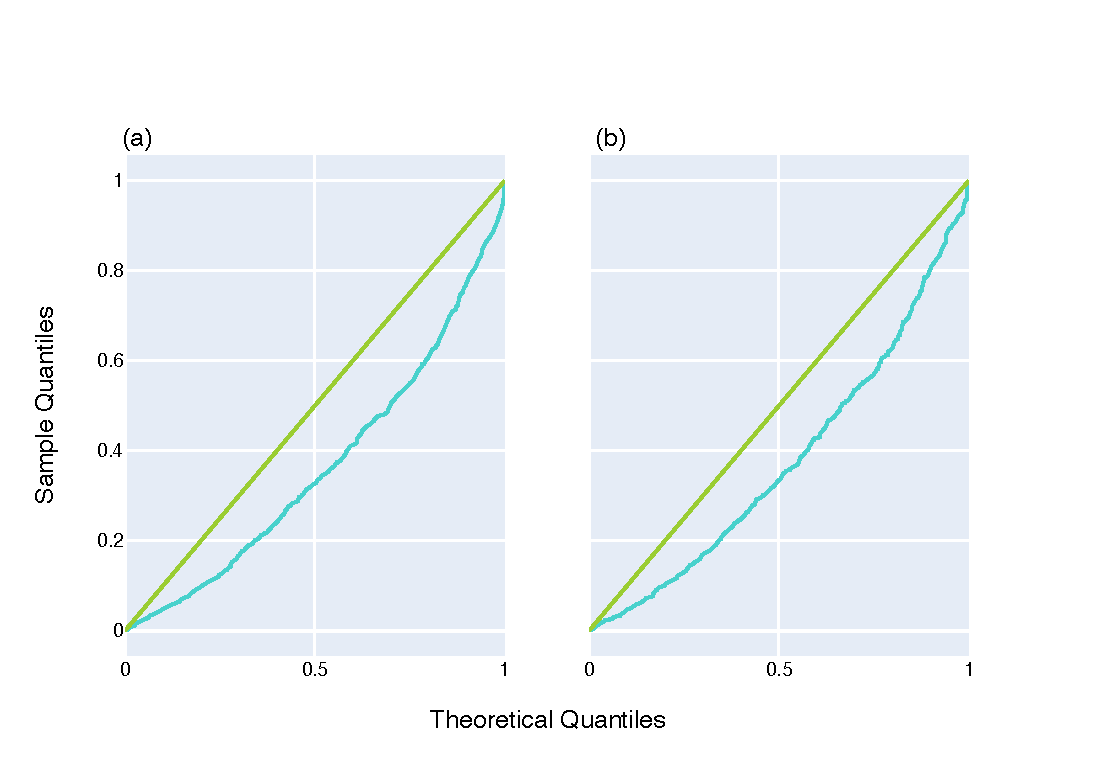
\includegraphics[width=\textwidth]{figures/plots/synthetic/lrt/197113_332182_17210-long_branch.pdf}
\caption{\textbf{Increasing the branch length to by a factor of 3 does not change the distribution of LRT p-values.} Quantile-Quantile plot comparing the distribution of the LRT p-values to the uniform distribution. \textbf{a}, simulated alignments of length 3000, \textbf{b}, simulated alignments of length 3000 with branch lengths scaled by a factor of 3. The data set was generated from the high JSD, high entropy seed.}
\label{fig:synthetic/lrt/197113-long_branch}
\end{figure}

\subsection{Published Tests}

\begin{figure}
\centering
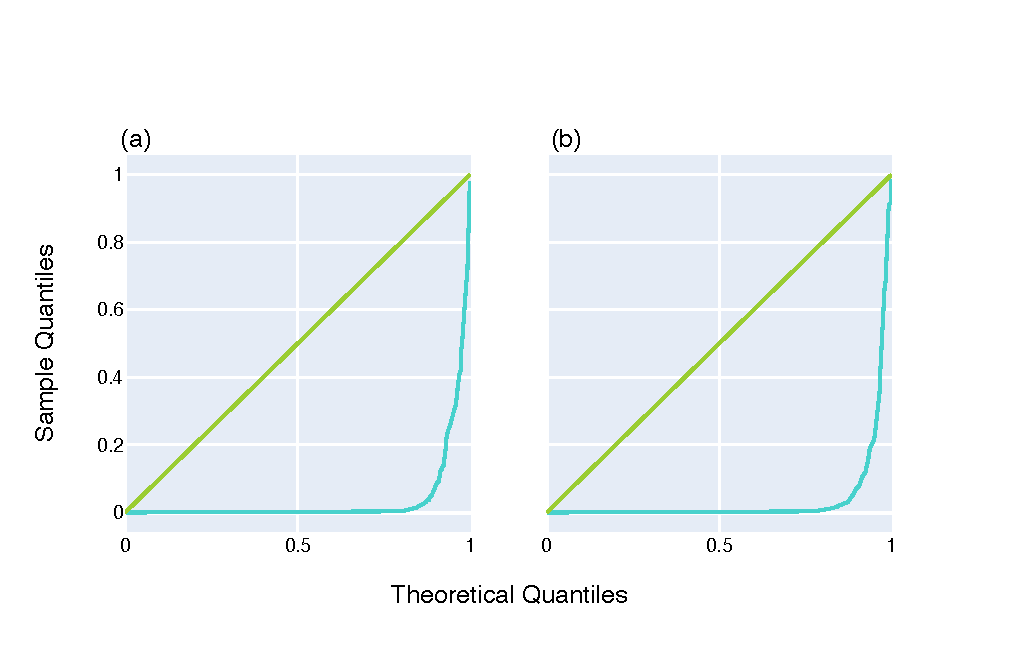
\includegraphics[width=\textwidth]{figures/plots/synthetic/chi2/197113_332182_17210.pdf}
\caption{}
\label{fig:synthetic/chi2}
\end{figure}

\subsection{$T_{50}$}

\begin{figure}[!ht]
\centering
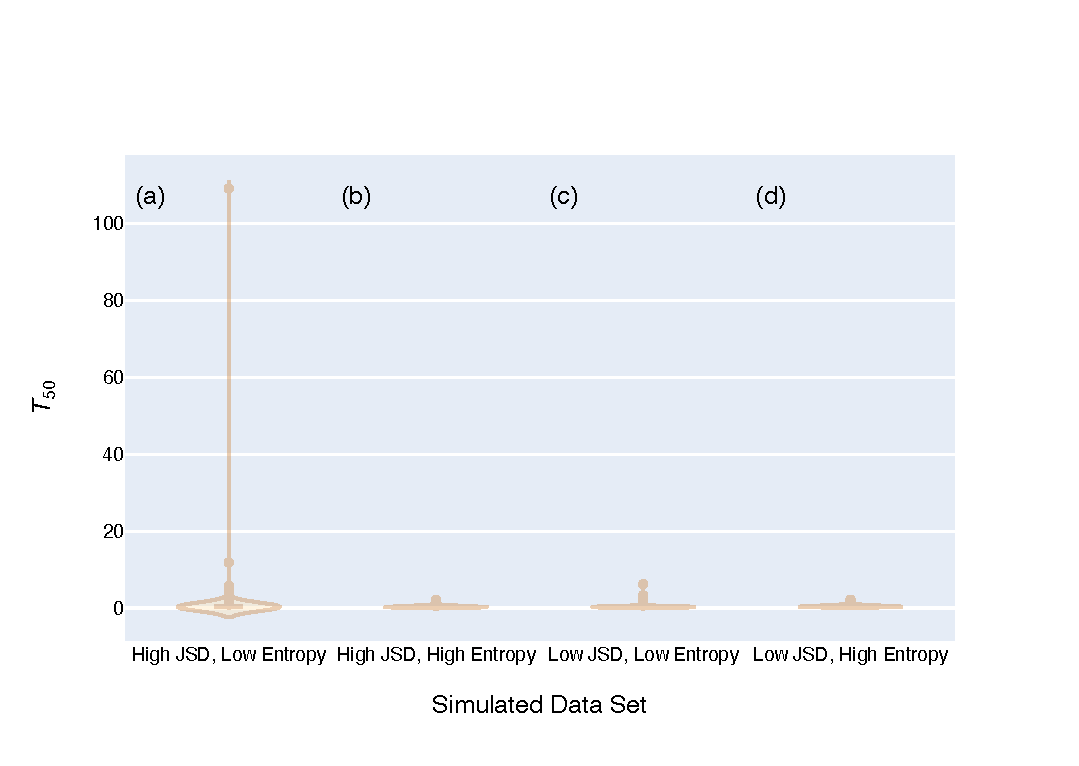
\includegraphics[width=\textwidth]{figures/plots/synthetic/T50/300bp.pdf}
\caption{\textbf{Low Entropy, High JSD data has sampling error for T50 estimates}}
\label{fig:t50_long}
\end{figure}

\begin{figure}[!ht]
\centering
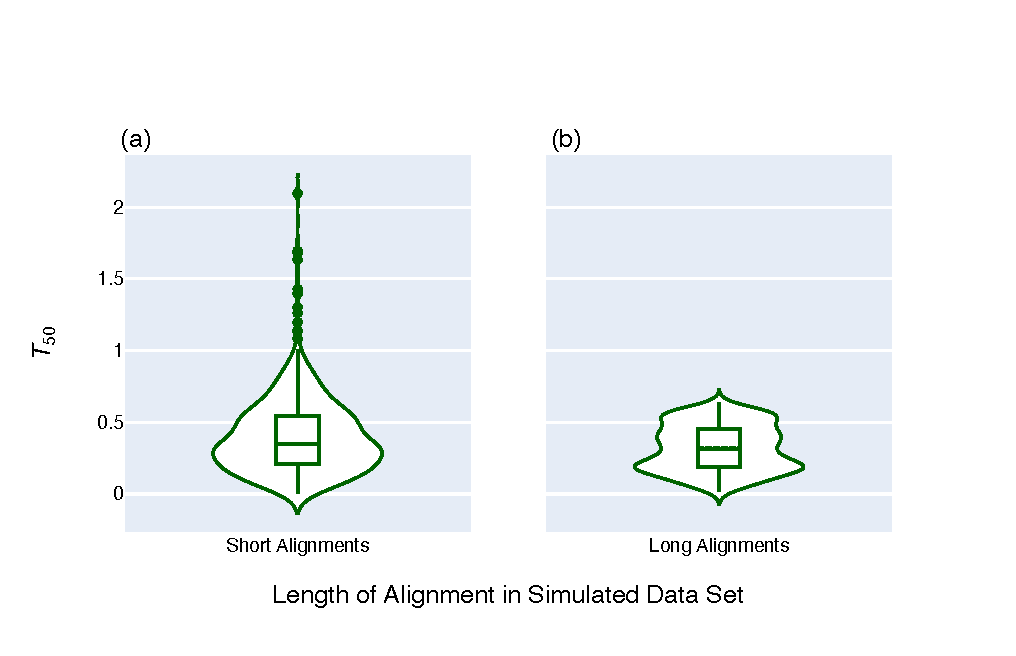
\includegraphics[width=\textwidth]{figures/plots/synthetic/T50/197113_332182_17210-seq_len.pdf}
\caption{\textbf{Long Alignments have less sampling error}}
\label{fig:T50-short_long}
\end{figure}

\subsection{Convergence}

\subsection{Equivalence of Process}

\section{Is the Human Genome at Equilibrium?}

\section{Is the \textit{D. melanogaster} genome further from equilibrium than \textit{D. simulans}?}

\section{Is the half of \textit{Fxy} located in the Psuedo-Autosomal Region (PAR) further from equilibrium than the non-PAR half in \textit{M. musculus}?}